\documentclass[8pt]{beamer}

% Beamer style
%\usetheme[secheader]{Madrid}
% \usetheme{CambridgeUS}
\useoutertheme{infolines}
\usecolortheme[rgb={0.65,0.15,0.25}]{structure}
% \usefonttheme[onlymath]{serif}
\beamertemplatenavigationsymbolsempty
%\AtBeginSubsection

% Packages
%\usepackage[french]{babel}
\usepackage[latin1]{inputenc}
\usepackage{color}
\usepackage{xspace}
\usepackage{dsfont, stmaryrd}
\usepackage{amsmath, amsfonts, amssymb}
\usepackage{epsfig}
\usepackage{tikz}
\usepackage{url}
% \usepackage{ulem}
\usepackage{/home/robin/LATEX/Biblio/astats}
%\usepackage[all]{xy}
\usepackage{graphicx}
\usepackage{xspace}

\input{/home/robin/RECHERCHE/EXPOSES/LATEX/Commands}
\newcommand{\CTSBM}{{\sl ct}-SBM\xspace}
\newcommand{\DTSBM}{{\sl dt}-SBM\xspace}

% Directory
\newcommand{\fignet}{/home/robin/Bureau/RECHERCHE/RESEAUX/EXPOSES/FIGURES}
\newcommand{\figchp}{/home/robin/Bureau/RECHERCHE/RUPTURES/EXPOSES/FIGURES}
\newcommand{\figfig}{../figs}


%====================================================================
%====================================================================

%====================================================================
%====================================================================
\begin{document}
%====================================================================
%====================================================================

%====================================================================
\title[Continuous time SBM]{A continuous	time SBM for time-stamped interactions}
  % (25 mn + 5 mn)

\author[S. Robin]{M. Ludkin$^1$, C. Matias$^2$, {\sl S. Robin}$^3$}

\institute[INRA/AgroParisTech/Paris-Saclay]{
  ($^1$) Lancaster University \\
  ($^2$) Sorbonne Universit\'es / CNRS \\
  ($^3$) INRA / AgroParisTech /univ. Paris-Saclay
  }

\date[SPA'18, Gothenburg]{Stochastic Processes and Applications, Gothenburg, Jun. 2018}

%====================================================================
%====================================================================
\maketitle
%====================================================================

%====================================================================
\frame{\frametitle{Outline} \tableofcontents}

%====================================================================
%====================================================================
\section{Time-stamped interaction data}
\frame{\frametitle{Outline} \tableofcontents[currentsection]}

%====================================================================
\frame{ \frametitle{Understanding network topology}

  \paragraph{Networks.}
  \begin{itemize}
   \item Popular way to encode interactions between entities
   \item Wide-range of applications: social sciences, biology, ecology, energy, etc
  \end{itemize}
  
  \pause \bigskip \bigskip
  \paragraph{Typical dataset.}
  \begin{itemize}
   \item $n$ nodes (individuals, species, genes, companies, etc.)
   \item $Y = (Y_{ij})_{1 \leq i, j \leq n}$ adjacency matrix:
   \begin{align*}
    Y_{ij} = \; & 1 & \text{if $i$ interacts with $j$} \\
    & 0 & \text{otherwise}
   \end{align*}
  \end{itemize}

  \pause \bigskip 
  \paragraph{Typical questions.}
  \begin{itemize}
   \item How is the network organized?
   \item Do all nodes play the same role?
  \end{itemize}
}

%====================================================================
\frame{ \frametitle{Stochastic block-model (SBM)}

  \paragraph{SBM \refer{HoL79,NoS01}:} one of the most popular models to analyze network heterogeneity (see also ERGM \refer{RPK07}).
  
  \bigskip
  \begin{tabular}{cc}
   \hspace{-.04\textwidth}
   \begin{tabular}{p{.65\textwidth}}
    \pause \paragraph{Model.}
    \begin{itemize}
     \item Nodes belong to $K$ groups: \\
     \tabequation{$(Z_i) \text{ iid } \sim \Mcal(1, \pi)$}
     \ra 'color', 'social role', ... \\ ~ 
     \item \pause Nodes interact with group-specific parameters: \\
     \tabequation{$(Y_{ij}) \text{ indep. } \gv (Z_i)$} 
     \tabequation{$Y_{ij} \gv (Z_i, Z_j) \sim \Bcal(\gamma_{Z_i, Z_j})$}
    \end{itemize}
   \end{tabular}
   & 
   \hspace{-.05\textwidth}
   \begin{tabular}{p{.35\textwidth}}
    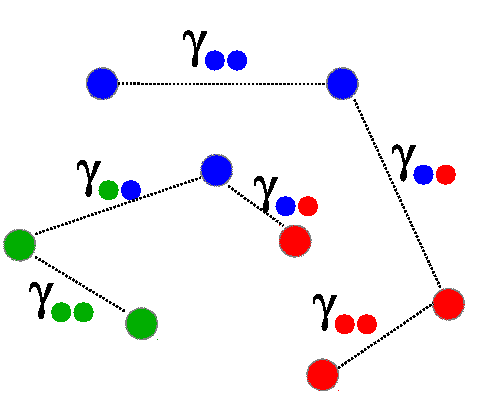
\includegraphics[width=.3\textwidth]{\fignet/FigSBM-Model-3-red}
   \end{tabular}
  \end{tabular}
  
  \bigskip
  \ra Node groups (colors) are not observed
}

%====================================================================
\frame{ \frametitle{Time-stamped interactions}

  \paragraph{Time-stamped data.}
  \begin{itemize}
   \item $n$ nodes
   \item $M$ time-stamped interaction triplets $(t_m, i_m, j_m)_{1\leq m \leq M}$:
   $$
   (t, i, j) = \{\text{\emphase{node $i$ interacts with node $j$ at time $t$}}\}
   $$
   (can be asymmetric: $i=$ sender, $j=$ receiver)
  \end{itemize}
  
  \pause \bigskip \bigskip
  \paragraph{Examples.} Animal interactions, emails, social contacts, ...

  \pause \bigskip \bigskip
  \paragraph{Questions.}
  \begin{itemize}
   \item Is the network topology stable \emphase{along time}?
   \item Do the nodes keep the same role \emphase{along time}?
  \end{itemize}

}

%====================================================================
\frame{ \frametitle{Continuous time SBM (\CTSBM)}

  \paragraph{Model.} \\~ 
  \begin{itemize}
   \item $n$ nodes, $K$ groups \\~ \\~ 
   \item \pause $Z_i = \{Z_i(t)\}_{0 \leq t \leq T}:$ group membership process of node $i$ belongs: 
   \begin{align*}
    (Z_i)_{1 \leq i \leq n} \text{ iid}
    \sim \text{ Markov jump process } (\nu, \lambda)
   \end{align*}
   $\nu =$ initial distribution, $\lambda = (\lambda_{k\ell})_{1 \leq k, \ell \leq K} =$ transition  rates \\ ~ \\ ~
   \item \pause $Y_{ij} = \{Y_{ij}(t)\}_{0\leq t \leq T}:$ interaction process between nodes $i$ and $j$: 
   \begin{align*}
    (Y_{ij})_{1 \leq i, j \leq n} & \text{ indep. } \gv (Z_i)_i, \qquad \\
    Y_{ij} \gv (Z_i, Z_j) & \sim \text{ heterogeneous Poisson process with rate $\gamma_{Z_i(t), Z_j(t)}$} 
   \end{align*}
  \end{itemize}
}

%====================================================================
\frame{ \frametitle{Proposed model}

  \vspace{-.1\textheight}
  \begin{overprint}
   \onslide<1> $$\includegraphics[height=.8\textheight,width=.8\textwidth]{\fignet/FigCTSBM-pathZ}$$
   \onslide<2> $$\includegraphics[height=.8\textheight,width=.8\textwidth]{\fignet/FigCTSBM-pathZY}$$
   \onslide<3> $$\includegraphics[height=.8\textheight,width=.8\textwidth]{\fignet/FigCTSBM-pathY}$$
  \end{overprint}
}

%====================================================================
%====================================================================
\section{Statistical inference}
\frame{\frametitle{Outline} \tableofcontents[currentsection]}

%====================================================================
\frame{ \frametitle{Further model specifications}

  \paragraph{Split time} into intervals $[t_{m-1}; t_m]$ ($t_0 = 0, t_{M+1}=T$)
  $$
  \Rightarrow \quad \forall i, j: \; \int_{t_{m-1}}^{t_m} \gamma_{Z_i(t), Z_j(t)} \d t 
  \simeq
  \frac{\delta_m}2 \sum_{k, \ell} \gamma_{k\ell} \left(Z_{ik}^{m-1} Z_{i\ell}^{m-1} + Z_{ik}^m Z_{i\ell}^m\right)
  $$
  where $Z_i^m = Z_i(t_m), Z_{ik}^m = \Ibb\{Z_i^m = k\}$. \pause
  \begin{itemize}
   \item All time intervals are considered (not only $(t_m, \emphase{i}, \emphase{j})$)
   \item Only need to deal with $Z_i^* = \{Z_i^m\}_{0 \leq m \leq M}$ (and not the full $Z_i$)
  \end{itemize}
  
  \pause \bigskip \bigskip 
  \paragraph{Transition rates.} Uniform transition
  $$
  \forall k: \qquad \lambda_{k\ell} = \lambda \; \nu_{\ell}
  $$
  \begin{itemize}
   \item Transition probability from $t_{m-1}$ to $t_m$ ($\delta_m = t_m - t_{m-1}$):
   $$
   \pi_m := \Pbb\{Z_i^m = \ell \gv Z_i^{m-1} = k\}
   = \nu_\ell \left(1 - e^{- \lambda \delta_m} \right) + \Ibb\{k = \ell\} e^{- \lambda \delta_m}
   $$
   \item Close form estimates (otherwise, numerical optimization is required)
  \end{itemize}
}

%====================================================================
\frame{ \frametitle{Inference for SBM-like models}

  \paragraph{Maximum likelihood.} 
  \begin{itemize}
   \item Want to estimate $\theta = (\nu, \lambda, \gamma)$
   \item $Z$ is not observed \ra \CTSBM = {\sl incomplete} data model
   \item Most popular strategy: Expectation-Maximization (EM \refer{DLR77})
  \end{itemize}
  
  \bigskip \bigskip \pause
  \paragraph{EM principle.} Based on the decomposition
  $$
  \log p_\theta(Y) = \Esp_\theta[\log p_\theta(Z, Y) \gv Y] - \Esp_\theta[\log p_\theta(Z \gv Y) \gv Y],
  $$
  consider only $\Esp_\theta[\log p_\theta(Z, Y) \gv Y]$ and iterate 
  \begin{itemize}
   \item \emphase{E-step:} compute some moments of $p_{\theta^h}(Z \gv Y)$ \qquad \qquad \quad (\emphase{'classification'}) 
   \item \emphase{M-step:} update $\theta^{h+1} = \arg\max_\theta \Esp_{\theta^h}[\log p_\theta(Z, Y) \gv Y]$ \qquad (\emphase{estimation}) 
  \end{itemize}
  
  \bigskip \bigskip \pause
  \paragraph{SBM-like models.} Due to graph moralization, the $Z_i$'s are not conditionally independent:
  $$
  p(Z_i, Z_j \gv Y_{ij}) \propto p(Z_i)  p(Z_j) p(Y_{ij} \gv Z_i, Z_j)
  $$
  \ra No factorization can be hoped to evaluate $p_\theta(Z \gv Y)$ in an efficient way\footnote{same for most heterogeneous graph models \refer{BJR07}}.

}

% %====================================================================
% \frame{ \frametitle{Inference for SBM-like models (2/2)}
% 
% 
%   \begin{tabular}{cc}
%     \begin{tabular}{p{.4\textwidth}}
% 	 EM requires to evaluate \\
% 	 \tabequation{$p_\theta(Z \gv Y)$}
% 	 
% 	 \onslide+<2->{
% 	 \bigskip
% 	 The $Z_i$'s are marginally independent \\
% 	 }
% 	 \onslide+<3->{
% 	 \bigskip
% 	 but conditionally all dependent
% 	 } \\~ \\~ \\~ \\~ \\~ 
%     \end{tabular}
%     & 
% %     \hspace{-.02\textwidth}
%     \begin{tabular}{p{.6\textwidth}}
% 	 \begin{overprint}
% 	  \onslide<2>\paragraph{Joint distribution:} $p(Z) p(Y \gv Z)$
% 	  \onslide<3>\paragraph{Joint distribution:} $p(Z \gv Y)$
% 	 \end{overprint} 
% 	 \\
% 	 \begin{overprint}
% 	  \onslide<2>\begin{tikzpicture}
\node[hidden] (Z1) at (0, \edgeunit) {$Z_1$};
\node[hidden] (Z2) at (\edgeunit, \edgeunit) {$Z_2$};
\node[hidden] (Z3) at (0, 0) {$Z_3$};
\node[hidden] (Z4) at (\edgeunit, 0) {$Z_4$};

\node[observed] (Y12) at (.5*\edgeunit, 1.75*\edgeunit) {$Y_{12}$};
\node[observed] (Y13) at (-.75*\edgeunit, .5*\edgeunit) {$Y_{13}$};
\node[observed] (Y14) at (1.75*\edgeunit, 1.75*\edgeunit) {$Y_{14}$};
\node[observed] (Y23) at (-.75*\edgeunit, 1.75*\edgeunit) {$Y_{23}$};
\node[observed] (Y24) at (1.75*\edgeunit, .5*\edgeunit) {$Y_{24}$};
\node[observed] (Y34) at (.5*\edgeunit, -.75*\edgeunit) {$Y_{34}$};

\draw[arrow] (Z1) to (Y12);  \draw[arrow] (Z2) to (Y12);
\draw[arrow] (Z1) to (Y13);  \draw[arrow] (Z3) to (Y13);
\draw[arrow] (Z1) to (Y14);  \draw[arrow] (Z4) to (Y14);
\draw[arrow] (Z2) to (Y23);  \draw[arrow] (Z3) to (Y23);
\draw[arrow] (Z2) to (Y24);  \draw[arrow] (Z4) to (Y24);
\draw[arrow] (Z3) to (Y34);  \draw[arrow] (Z4) to (Y34);
\end{tikzpicture}

% 	  \onslide<3>\begin{tikzpicture}
\node[hidden] (Z1) at (0, \edgeunit) {$Z_1$};
\node[hidden] (Z2) at (\edgeunit, \edgeunit) {$Z_2$};
\node[hidden] (Z3) at (0, 0) {$Z_3$};
\node[hidden] (Z4) at (\edgeunit, 0) {$Z_4$};

\node[eliminated] (Y12) at (.5*\edgeunit, 1.75*\edgeunit) {$Y_{12}$};
\node[eliminated] (Y13) at (-.75*\edgeunit, .5*\edgeunit) {$Y_{13}$};
\node[eliminated] (Y14) at (1.75*\edgeunit, 1.75*\edgeunit) {$Y_{14}$};
\node[eliminated] (Y23) at (-.75*\edgeunit, 1.75*\edgeunit) {$Y_{23}$};
\node[eliminated] (Y24) at (1.75*\edgeunit, .5*\edgeunit) {$Y_{24}$};
\node[eliminated] (Y34) at (.5*\edgeunit, -.75*\edgeunit) {$Y_{34}$};

\draw[edge] (Z1) to (Z2);  \draw[edge] (Z1) to (Z3);
\draw[edge] (Z1) to (Z4);  \draw[edge] (Z2) to (Z3);
\draw[edge] (Z2) to (Z4);  \draw[edge] (Z3) to (Z4);

\draw[lightarrow] (Z1) to (Y12);  \draw[lightarrow] (Z2) to (Y12);
\draw[lightarrow] (Z1) to (Y13);  \draw[lightarrow] (Z3) to (Y13);
\draw[lightarrow] (Z1) to (Y14);  \draw[lightarrow] (Z4) to (Y14);
\draw[lightarrow] (Z2) to (Y23);  \draw[lightarrow] (Z3) to (Y23);
\draw[lightarrow] (Z2) to (Y24);  \draw[lightarrow] (Z4) to (Y24);
\draw[lightarrow] (Z3) to (Y34);  \draw[lightarrow] (Z4) to (Y34);
\end{tikzpicture}

% 	 \end{overprint}
%     \end{tabular}
%   \end{tabular}
% 
%   \bigskip
%   \onslide+<3> \ra No factorization can be hoped to evaluate $p_\theta(Z \gv Y)$ in an efficient way.
% }

%====================================================================
\frame{ \frametitle{Inference for \CTSBM}

  \paragraph{Variational inference \refer{WaJ08,BKM17}.} Maximize a lower bound\footnote{$KL[q||p] = \Esp_q \log(q/p)$ for $q \gg p$}  of $\log p_\theta(Y)$:
  \begin{align*}
    J(\theta, q) 
    = \log p_\theta(Y) \emphase{- KL[q(Z) \ggv  p_\theta(Z \gv Y)]}
    = \Esp_q[\log p_\theta(Z, Y)] - \Esp_q[\log q(Z)]
  \end{align*}
  for $q \in \Qcal$
  \ra \emphase{Variational EM} (VEM)
  
  \pause \bigskip \bigskip 
  \paragraph{Distribution class $\Qcal$.} 
  \begin{itemize}
   \item Balance between approximation quality and mathematical ease
   \item Standard choice for SBM-like models \refer{DPR08}
   $$
   \Qcal = \left\{q: q(Z) = \prod_{i=1}^n q_i(Z_i)\right\}.
   $$
  \end{itemize}
}

%====================================================================
\frame{ \frametitle{Variational EM}

  The objective function
  $$
  \Esp_q[\log p_\theta(Z^*, Y)]
  $$
  involves $q(Z_i^m)$, $q(Z_i^{m-1} ,Z_i^m)$, $q(Z_i^m, Z_j^m)$.

  \pause \bigskip \bigskip
  \paragraph{VE-step.} Determine the optimal approximate distribution $q^h(Z^*) \approx p_{\theta^h}(Z^* \gv Y)$ 
  \begin{itemize}
   \item Because $q$ factorizes, $q(Z_i^m, Z_j^m) = q(Z_i^m) q(Z_j^m)$ 
   \item Minimizing $KL$: $q_i =$ heterogeneous continuous times Markov process 
   \item $q(Z_i^m)$, $q(Z_i^{m-1} ,Z_i^m)$ computed via forward-backward recursion \refer{JuR91}
  \end{itemize}
  \ra Similar to coupled HMM \refer{Mur02}

  \pause \bigskip \bigskip
  \paragraph{M-step.} Maximize the objective function wrt $\theta$ 
  \begin{itemize}
   \item Existence and uniqueness for the updates $\theta^h = (\nu^h, \lambda^h, \gamma^h)$ 
  \end{itemize}
}

%====================================================================
\frame{ \frametitle{Model selection}

  \paragraph{Popular criteria} adapted to \CTSBM 
  \begin{itemize}
   \item $BIC$ \refer{Sch78}: Laplace approximation of $p(K \gv Y)$:
   $$
   BIC(K) = \log p_{\widehat{\theta}, K}(Y) - \frac12 K \log(nM) - \frac12 K^2 \log(M)
   $$
   \item $ICL$ \refer{BCG00}: for classification purposed, penalize for $\Hcal(Z \gv Y)$:
   $$
   ICL(K) = BIC(K) - \Hcal(Z \gv Y)
   $$
  \end{itemize}
  
  \bigskip 
  \paragraph{Variational approximation.} Replace $\log p_{\widehat{\theta}}(Y)$ with its lower bound $J(\widehat{\theta}, \widehat{q})$

}

%====================================================================
\section{Simulations and Illustrations}
\frame{\frametitle{Outline} \tableofcontents[currentsection]}

%====================================================================
\frame{ \frametitle{Simulation study}

  \begin{tabular}{cc}
    \hspace{-.05\textwidth}
    \begin{tabular}{p{.4\textwidth}}
	 \paragraph{Simulation design.} $K =$ 3 groups \\ ~
	 \begin{itemize}
	 \item $G =$ expected number of interactions / pair / unit time \\ ~
	 \item $R =$ expected number of changes / node / unit time \\ ~
	 \item $D =$ scale between within and between-group interaction rates \\ ~
	 \item caption: $G$\_$R$\_$D$ \\~
	 \end{itemize}
    \end{tabular}
    & 
    \hspace{-.075\textwidth}
    \begin{tabular}{p{.6\textwidth}}
	 \begin{overprint}
	  \onslide<2> \includegraphics[width=.6\textwidth, height=.7\textheight]{\fignet/ctSBM-sim-ARI}
	  \onslide<3> \includegraphics[width=.6\textwidth, height=.7\textheight]{\fignet/ctSBM-sim-ICL}
	 \end{overprint}
    \end{tabular}
  \end{tabular}  
}

%====================================================================
\frame{ \frametitle{Zebra dynamic social network \refer{RSF15}}

  \begin{tabular}{cc}
%     \hspace{-.05\textwidth}
    \begin{tabular}{p{.45\textwidth}}
	\begin{itemize}
	 \item $n = 26$ zebras \\ ~
	 \item 26 days \\ ~
	 \item $M \simeq 900$ interactions \\ ~
	 \item 4 types: \textcolor{cyan}{bachelor}, \textcolor{pink}{lactating}, \textcolor{yellow}{non-lactating}, \textcolor{gray}{stallion}, 
	\end{itemize}
	
	\bigskip
	\onslide+<2->{
	 \paragraph{Estimates.} $1000 \; \widehat{\lambda} = 242.6$ \\ ~ \\
	 {
	   $
	   \begin{array}{lcccc}
	    & & \textcolor{red}{1} & \textcolor{green}{2} & \textcolor{blue}{3} \\
	   \hline 
	   \widehat{\nu} &  & 0.091 & 0.200 & 0.709 \\
	   \hline
	   & \textcolor{red}{1} & 209.6 & 0.300 & 0.007 \\
	   1000 \; \widehat{\gamma} & \textcolor{green}{2} & 0.300 & 304.1 & 0.033 \\
	   & \textcolor{blue}{3} & 0.007 & 0.034 & 1.345 \\
	   \end{array}
	   $
	 }} \\~ \\~ 
% > round(lambda, 3); round(nu, 3); round(1000*gamma, 3)
% [1] 0.242
% [1] 0.091 0.200 0.709
%         [,1]    [,2]  [,3]
% [1,] 209.585   0.300 0.007
% [2,]   0.300 304.119 0.033
% [3,]   0.007   0.034 1.345
\end{tabular}
    & 
    \hspace{-.1\textwidth}
    \begin{tabular}{p{.5\textwidth}}
	 \begin{overprint}
	 \onslide<1> \includegraphics[width=.5\textwidth]{\fignet/ctSBM-zebra-modsel}
	 \onslide<2> \includegraphics[width=.5\textwidth]{\fignet/ctSBM-zebra-path}
	 \end{overprint}
    \end{tabular}
  \end{tabular}
}

%====================================================================
%====================================================================
\section{Conclusion \& Future works}
% \frame{\frametitle{Outline} \tableofcontents[currentsection]}

%====================================================================
\frame{ \frametitle{Conclusion \& Future works}

  \pause 
  \paragraph{Related works:} Dynamic SBMs
  \begin{itemize}
   \item Discrete time (\DTSBM): mixed-membership \refer{XFS10,HSX15}, duration \refer{Xu15}, \refer{XuH14}, identifiability \refer{MaM16}
   \item Continuous time: limited interaction times \refer{CLR17}, \refer{LFM16}
  \end{itemize}
  \ra All rely on variational approximations, or MCMC, or both


  \pause \bigskip \bigskip 
  \paragraph{Our contribution.}
  \begin{itemize}
  \item A continuous time version of SBM: \CTSBM
  \item A variational EM algorithm for its inference
  \end{itemize}
  
  \pause \bigskip \bigskip 
  \paragraph{Further works.}
  \begin{itemize}
   \item Accounting for covariates
   \item Identifiability: holds for SBM~\refer{AMR09} and \DTSBM~\refer{MaM16}
   \item Statistical guarantees for VEM estimates \\ 
   \ra Consistency for SBM \refer{CDP12,BCC13,MaM15}, but extension to \CTSBM unclear \\
   \ra Starting point for statistically grounded, but computationally demanding inference
  \end{itemize}
}

%====================================================================
\frame[allowframebreaks]{ \frametitle{References}
  {%\footnotesize
   \tiny
   \bibliography{/home/robin/Biblio/BibGene}
%    \bibliographystyle{/home/robin/LATEX/Biblio/astats}
   \bibliographystyle{alpha}
  }
}


%====================================================================
\appendix 
\backupbegin
\section{Backup}
\frame{\frametitle{Outline} \tableofcontents[currentsection]}

%====================================================================
\frame{ \frametitle{Graph moralization}

  \begin{overprint}
   \onslide<1>
   $$
  \begin{tikzpicture}
  \node[hidden] (Z1) at (0, \edgeunit) {$Z_1$};
  \node[hidden] (Z2) at (\edgeunit, \edgeunit) {$Z_2$};
  \node[hidden] (Z3) at (0, 0) {$Z_3$};
  \node[hidden] (Z4) at (\edgeunit, 0) {$Z_4$};

  \node[observed] (Y12) at (.5*\edgeunit, 1.75*\edgeunit) {$Y_{12}$};
  \node[observed] (Y13) at (-.75*\edgeunit, .5*\edgeunit) {$Y_{13}$};
  \node[observed] (Y14) at (1.75*\edgeunit, 1.75*\edgeunit) {$Y_{14}$};
  \node[observed] (Y23) at (-.75*\edgeunit, 1.75*\edgeunit) {$Y_{23}$};
  \node[observed] (Y24) at (1.75*\edgeunit, .5*\edgeunit) {$Y_{24}$};
  \node[observed] (Y34) at (.5*\edgeunit, -.75*\edgeunit) {$Y_{34}$};
  
  \draw[arrow] (Z1) to (Y12);  \draw[arrow] (Z2) to (Y12);
  \draw[arrow] (Z1) to (Y13);  \draw[arrow] (Z3) to (Y13);
  \draw[arrow] (Z1) to (Y14);  \draw[arrow] (Z4) to (Y14);
  \draw[arrow] (Z2) to (Y23);  \draw[arrow] (Z3) to (Y23);
  \draw[arrow] (Z2) to (Y24);  \draw[arrow] (Z4) to (Y24);
  \draw[arrow] (Z3) to (Y34);  \draw[arrow] (Z4) to (Y34);
  \end{tikzpicture}
  $$
  \onslide<2>
  $$
  \begin{tikzpicture}
  \node[hidden] (Z1) at (0, \edgeunit) {$Z_1$};
  \node[hidden] (Z2) at (\edgeunit, \edgeunit) {$Z_2$};
  \node[hidden] (Z3) at (0, 0) {$Z_3$};
  \node[hidden] (Z4) at (\edgeunit, 0) {$Z_4$};

  \node[eliminated] (Y12) at (.5*\edgeunit, 1.75*\edgeunit) {$Y_{12}$};
  \node[eliminated] (Y13) at (-.75*\edgeunit, .5*\edgeunit) {$Y_{13}$};
  \node[eliminated] (Y14) at (1.75*\edgeunit, 1.75*\edgeunit) {$Y_{14}$};
  \node[eliminated] (Y23) at (-.75*\edgeunit, 1.75*\edgeunit) {$Y_{23}$};
  \node[eliminated] (Y24) at (1.75*\edgeunit, .5*\edgeunit) {$Y_{24}$};
  \node[eliminated] (Y34) at (.5*\edgeunit, -.75*\edgeunit) {$Y_{34}$};
  
  \draw[edge] (Z1) to (Z2);  \draw[edge] (Z1) to (Z3);
  \draw[edge] (Z1) to (Z4);  \draw[edge] (Z2) to (Z3);
  \draw[edge] (Z2) to (Z4);  \draw[edge] (Z3) to (Z4);
  
    
  \draw[lightarrow] (Z1) to (Y12);  \draw[lightarrow] (Z2) to (Y12);
  \draw[lightarrow] (Z1) to (Y13);  \draw[lightarrow] (Z3) to (Y13);
  \draw[lightarrow] (Z1) to (Y14);  \draw[lightarrow] (Z4) to (Y14);
  \draw[lightarrow] (Z2) to (Y23);  \draw[lightarrow] (Z3) to (Y23);
  \draw[lightarrow] (Z2) to (Y24);  \draw[lightarrow] (Z4) to (Y24);
  \draw[lightarrow] (Z3) to (Y34);  \draw[lightarrow] (Z4) to (Y34);
  \end{tikzpicture}
  $$
  \end{overprint}
}

%====================================================================
\frame{ \frametitle{Primary school}

  \begin{tabular}{cc}
%     \hspace{-.05\textwidth}
    \begin{tabular}{p{.5\textwidth}}
	\begin{itemize}
	 \item $n = 84$ children, $M \simeq 539$ interactions over 3 hours \\ ~
	 \item 4 classes: \textcolor{yellow}{1A}, \textcolor{gray}{2A}, \textcolor{black}{4A}, \textcolor{red}{5A}, 
	\end{itemize}
	
	\bigskip
	\onslide+<2->{
	 \paragraph{Estimates.} $\widehat{\lambda} = 0.4.35$  1e4 \\ ~ \\
	 {\tiny
	   $
	   \begin{array}{lcccccc}
	    & & \textcolor{red}{1} & \textcolor{green}{2} & \textcolor{blue}{3} & \textcolor{cyan}{4} & \textcolor{pink}{5} \\
	   \hline 
	   \widehat{\nu} &  & 0.138 & 0.105 & 0.133 & 0.149 & 0.475 \\
	   \hline
	   & \textcolor{red}{1}   & 0.183 & 0.019 & 2.653 & 0.019 & 0.016 \\
	   1e3 & \textcolor{green}{2} & 0.002 & 0.229 & 0.027 & 0.000 & 0.000 \\
	   \widehat{\gamma} & \textcolor{blue}{3} & 0.012 & 0.009 & 0.132 & 0.002 & 0.003 \\
	   & \textcolor{cyan}{4}  & 0.002 & 0.000 & 0.008 & 0.375 & 0.002 \\
	   & \textcolor{pink}{5}  & 0.008 & 0.000 & 0.005 & 0.005 & 0.026 \\
	   \end{array}
	   $
	 }} \\~ \\~ 
% > round(1000*lambda, 3); round(nu, 3); round(1000*gamma, 3)
% [1] 0.435
% [1] 0.138 0.105 0.133 0.149 0.475
%       [,1]  [,2]  [,3]  [,4]  [,5]
% [1,] 
% [2,] 
% [3,] 
% [4,] 
% [5,] 
\end{tabular}
    & 
    \hspace{-.1\textwidth}
    \begin{tabular}{p{.5\textwidth}}
	 \begin{overprint}
	 \onslide<1> \includegraphics[width=.5\textwidth]{\fignet/ctSBM-primaryschool-modsel}
	 \onslide<2> 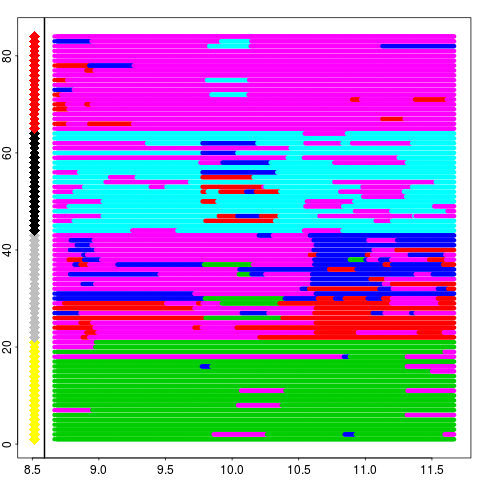
\includegraphics[width=.5\textwidth]{\fignet/ctSBM-primaryschool-path}
	 \end{overprint}
    \end{tabular}
  \end{tabular}

}

\backupend

%====================================================================
%====================================================================
\end{document}
%====================================================================
%====================================================================

  \begin{tabular}{cc}
    \begin{tabular}{p{.5\textwidth}}
    \end{tabular}
    & 
    \hspace{-.02\textwidth}
    \begin{tabular}{p{.5\textwidth}}
    \end{tabular}
  \end{tabular}

